\documentclass[a4paper, 12pt]{article}
\usepackage[top=1cm, bottom = 2cm, left = 2cm, right = 2cm]{geometry}
\usepackage[utf8]{inputenc}
\usepackage[brazil]{babel}
\usepackage{listings}
\usepackage[framed, numbered]{matlab-prettifier}
\usepackage[T1]{fontenc}
\usepackage{indentfirst}
\usepackage{graphicx}
\usepackage{epstopdf}
\usepackage{float}
\usepackage{amsmath}
\usepackage{amssymb}
\usepackage{systeme}

\title{Exercício 3 - Aula 4 \\ EET-01}

\author{
  Igor Caldeira Magalhães\\igorcmag@gmail.com
}
\date{08 de maio de 2020}

\begin{document}
\maketitle
\section{Enunciado}

Verifique graficamente (matalab ou octave) as propriedades da Transformada de Fourier apresentadas em aula.

%O exercício deve ser entregue: Documento simples deve ser apresentado, contendo o seguinte conteúdo:
%Nome da disciplina;
%Nome do aluno;
%Enunciado do exercício;
%Figuras obtidas - Com breve descrição: A Figura xx mostra ...
%Código .m e breve descrição do código matlab (octave);

\section{Solução}

\lstinputlisting[style=Matlab-editor, caption={Código em MATLAB para gerar todas as sequências do exercício, bem como suas transformadas de Fourrier de tempo discreto e seus gráficos.}, basicstyle = \mlttfamily\scriptsize]{ex3.m}

\begin{figure}[H]
	\centering
	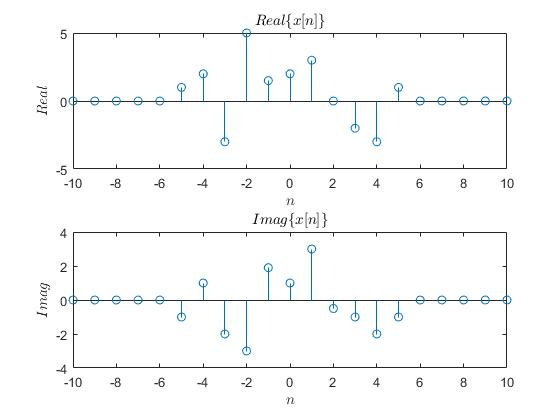
\includegraphics[scale=0.7]{img1.jpg} 
	\caption{Gráfico do sinal $x[n]$ que será usado de exemplo para verificação das propriedades.}
	\label{fig:1}
\end{figure}

\begin{figure}[H]
	\centering
	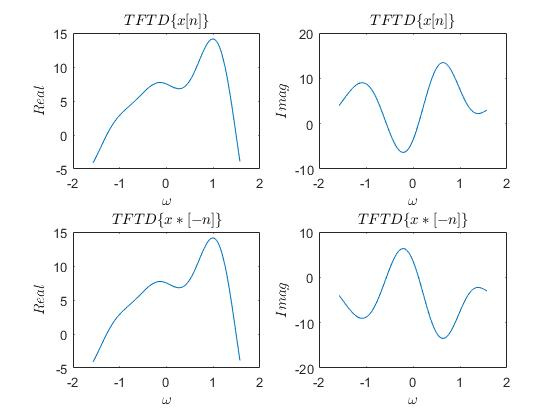
\includegraphics[scale=0.7]{img2.jpg} 
	\caption{Verificação da primeira propriedade de simetria. Observa-se que $TFTD*\lbrace x[n]\rbrace = TFTD\lbrace x*[-n]\rbrace$}
	\label{fig:2}
\end{figure}

\begin{figure}[H]
	\centering
	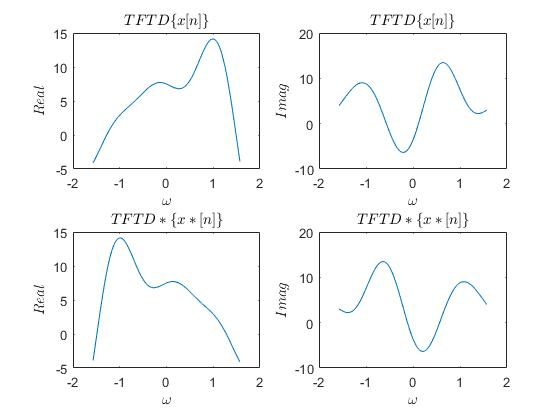
\includegraphics[scale=0.7]{img3.jpg} 
	\caption{Verificação da segunda propriedade de simetria. Observa-se que $TFTD\lbrace x[n]\rbrace (\omega ) = TFTD*\lbrace x*[-n]\rbrace (-\omega )$}
	\label{fig:3}
\end{figure}

\begin{figure}[H]
	\centering
	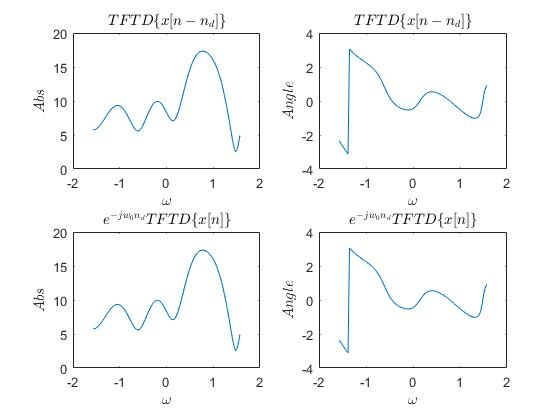
\includegraphics[scale=0.7]{img4.jpg} 
	\caption{Verificação de deslocamento no tempo. Observa-se que $TFTD \lbrace x[n-n_d]\rbrace = e^{-jw_0n_d}TFTD \lbrace x[n]\rbrace$}
	\label{fig:4}
\end{figure}

\begin{figure}[H]
	\centering
	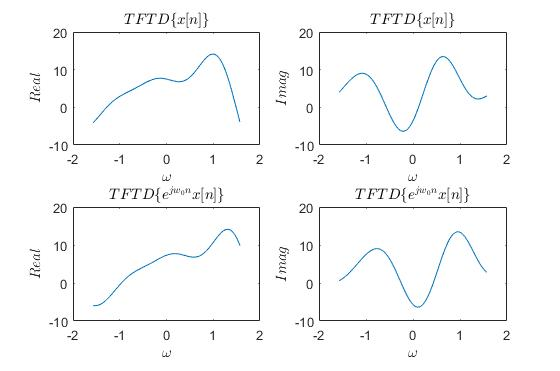
\includegraphics[scale=0.7]{img5.jpg} 
	\caption{Verificação de deslocamento em frequência. Observa-se que $TFTD \lbrace x[n]\rbrace (\omega - \omega_0 ) = TFTD \lbrace e^{jw_0n}x[n]\rbrace (\omega )$}
	\label{fig:5}
\end{figure}

\begin{figure}[H]
	\centering
	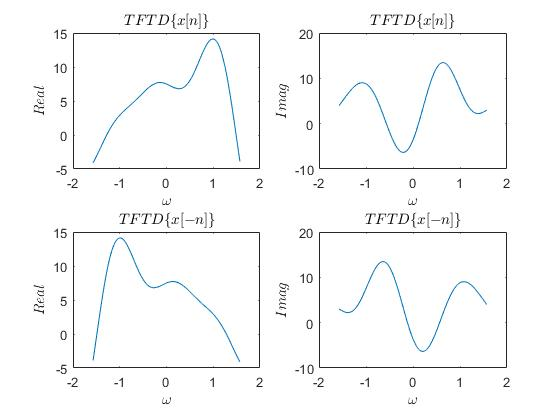
\includegraphics[scale=0.7]{img6.jpg} 
	\caption{Verificação de reversão no tempo. Observa-se que $TFTD \lbrace x[n]\rbrace (\omega) = TFTD \lbrace x[-n]\rbrace (-\omega )$}
	\label{fig:6}
\end{figure}

\begin{figure}[H]
	\centering
	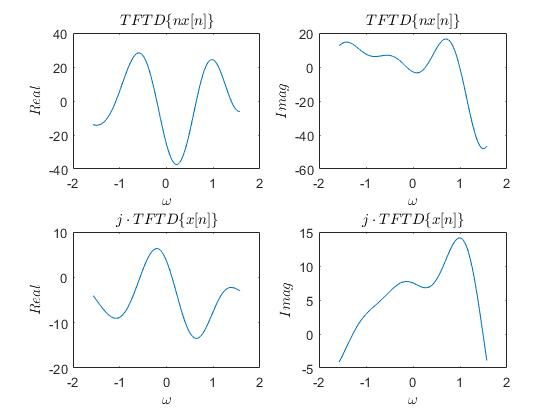
\includegraphics[scale=0.7]{img7.jpg} 
	\caption{Verificação de diferenciação em frequência. Observa-se que $TFTD \lbrace nx[n]\rbrace = \frac{d}{d\omega}j\cdot TFTD \lbrace x[n]\rbrace$}
	\label{fig:7}
\end{figure}

\end{document}